\documentclass[a4paper,12pt]{article}

\title{Physics 30 \\ Electromagnetic Radiation - Optics}
\author{Jad Chehimi}

% document setup
\renewcommand{\familydefault}{\sfdefault}
\linespread{1.25}
\usepackage[margin=1in]{geometry}
\usepackage{setspace}
\usepackage{enumitem}
\setlist{nosep}
\usepackage{color,soul}
\setcounter{secnumdepth}{0}

% tools
\usepackage[hidelinks]{hyperref}
\usepackage{float}
%% images
\usepackage{graphicx}
\graphicspath{ {./images/} }
%% science
\usepackage{siunitx}
\sisetup{exponent-product=\times, per-mode=fraction}

\begin{document}
\maketitle

% temp
\begin{center}
\Huge
Unfinished!
\normalsize
\end{center}
% temp

\tableofcontents

\pagebreak

\section{Terms}
\begin{itemize}
    \item{\textbf{Monochromatic Light}: Light of one colour}
    \item{\textbf{Medium}: the material the wave is travelling in}
    \item{\textbf{Refraction}: a change in the direction of a light wave due to a change in its speed as it passes from one medium to another}
    \item{\textbf{Refractive Index}: a ratio comparing the speed of light in a vacuum to the measured speed of light in a given material ($n = \frac{c}{v}$)}
\end{itemize}

\section{Electromagnetic Spectrum}
\begin{figure}[H]
    \centering
    \caption{"Cosmic" rays on the left of gamma}
    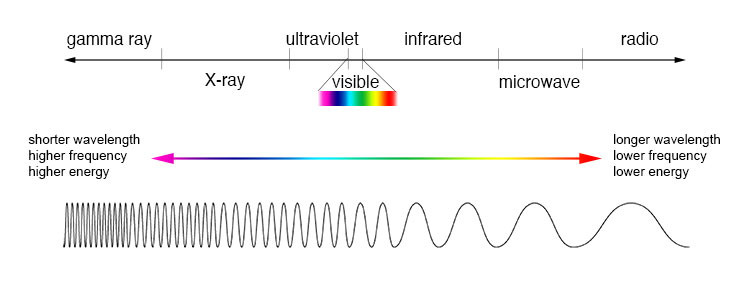
\includegraphics[width=\textwidth]{emr}
\end{figure}
\begin{itemize}
    \item{ALL EMR travels at the speed of light. ($c = \SI{3.00e8}{\m\per\s}$)}
    \item{
        \hl{Memorize the visible spectrum wavelength range}
        \begin{itemize}
            \item{\SI{400}{\nano\m} to \SI{750}{\nano\m}}
            \item{\SI{400e-9}{\m} to \SI{750e-9}{\m}}
        \end{itemize}
    }
\end{itemize}

\subsection{Universal Wave Equation}
\Large $$v = f\lambda$$ \normalsize
\begin{itemize}
    \item{$v$ = speed (\si{\m\per\s})}
    \item{$f$ = frequency (\si{\Hz})}
    \item{$\lambda$ = wavelength (\si{\m}) (often given in nanometers, $\SI{100}{\nano\m} = \SI{100e-9}{\m}$)}
\end{itemize}

Speed of light: $c = f\lambda$

\subsection{Transverse Wave}
\begin{figure}[H]
    \centering
    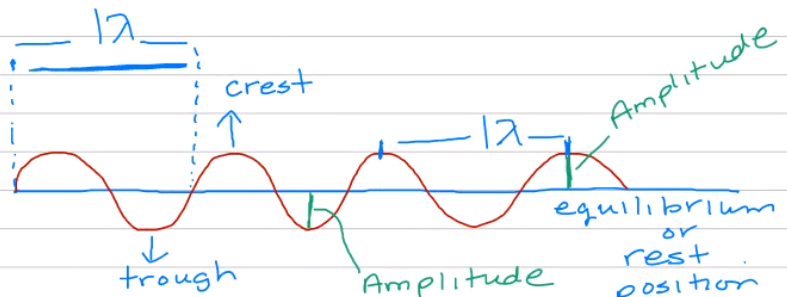
\includegraphics[width=0.9\textwidth]{transverse}
\end{figure}
\begin{itemize}
    \item{\textbf{Crest}: peak of wave}
    \item{\textbf{Trough}: depression of wave}
    \item{\textbf{Amplitude}: the maximum displacement from the equilibrium position}
\end{itemize}

\section{Law of Reflection}

\Large $$\angle{I} = \angle{R}$$ \normalsize

\begin{figure}[H]
    \centering
    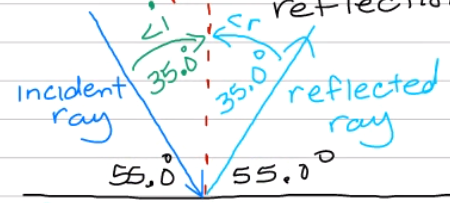
\includegraphics[width=0.50\textwidth]{reflect}
\end{figure}

\begin{itemize}
    \item{$\angle{I}$: \textbf{Angle of Incidence} \\Measured from the light ray to the normal}
    \item{$\angle{R}$: \textbf{Angle of Reflection} \\Measured from reflected ray to normal}
    \item{
            \textbf{Normal}
            \begin{itemize}
                \item{Perpendicular to the surface}
                \item{Broken/dotted line}
                \item{Drawn from where the incident ray contacts the mirror surface}
            \end{itemize}
        }
\end{itemize}

\subsection{Example}
A light ray strikes a flat mirror at an angle of \ang{70.0} to the mirror surface. What is the angle of reflection? What is the angle between the incident ray and the reflected ray?
\begin{figure}[H]
    \centering
    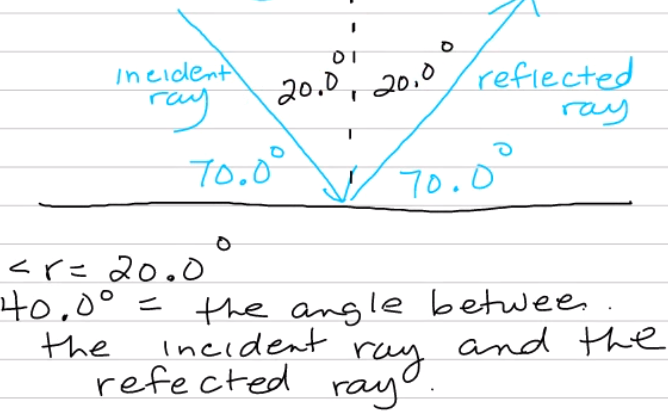
\includegraphics[width=0.6\textwidth]{ex-reflect}
\end{figure}

\section{Refraction}
The bending of a wave when entering a new medium at an angle.

\begin{itemize}
    \item{$n$: Index of Refraction (air is $n = \num{1.00}$)}
    \item{When a light ray travels from a lower $n$-value medium to a greater $n$-value medium, the light ray will \hl{bend toward the normal}}
\end{itemize}

\subsection{Snell's Law}
\Large $$n_1\sin{\theta_1} = n_2\sin{\theta_2}$$ \normalsize
Use to calculate the new angle in a different medium/n value.

\Large $$\frac{n_2}{n_1} = \frac{\sin{\theta_1}}{\sin{\theta_2}} = \frac{\lambda_1}{\lambda_2} = \frac{v_1}{v_2}$$ \normalsize

\subsection{Frequency}
Frequency is \hl{unaffected by medium}. 

Frequency can only be changed at the source.

\subsection{Critical Angle}
For any two mediums, the critical angle is the angle of the incident angle for which the angle of refraction is \ang{90}.

Two conditions must be met for a critical angle.
\begin{itemize}
    \item{The light must travel from a \hl{greater $n$-value to a lesser $n$-value}}
    \item{The angle of refraction must be \ang{90.0}}
\end{itemize}
\begin{figure}[H]
    \centering
    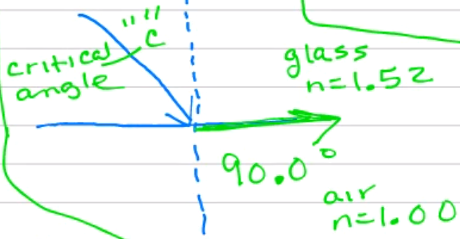
\includegraphics[width=0.50\textwidth]{criticalangle}
\end{figure}

\subsection{Total Internal Reflection}
Reflection of all incident light back into a medium of higher refractive index due to the inability to refract light back at an angle beyond the maximum angle of \ang{90}.

If the angle of incidence is \hl{greater than the critical value}, then the ray will \hl{reflect instead of refract}. (therefore, staying inside the medium)

Trying to calculate this angle with Snell's Law will error.

\subsection{Examples}
\subsubsection{Parallelogram}
\begin{figure}[H]
    \centering
    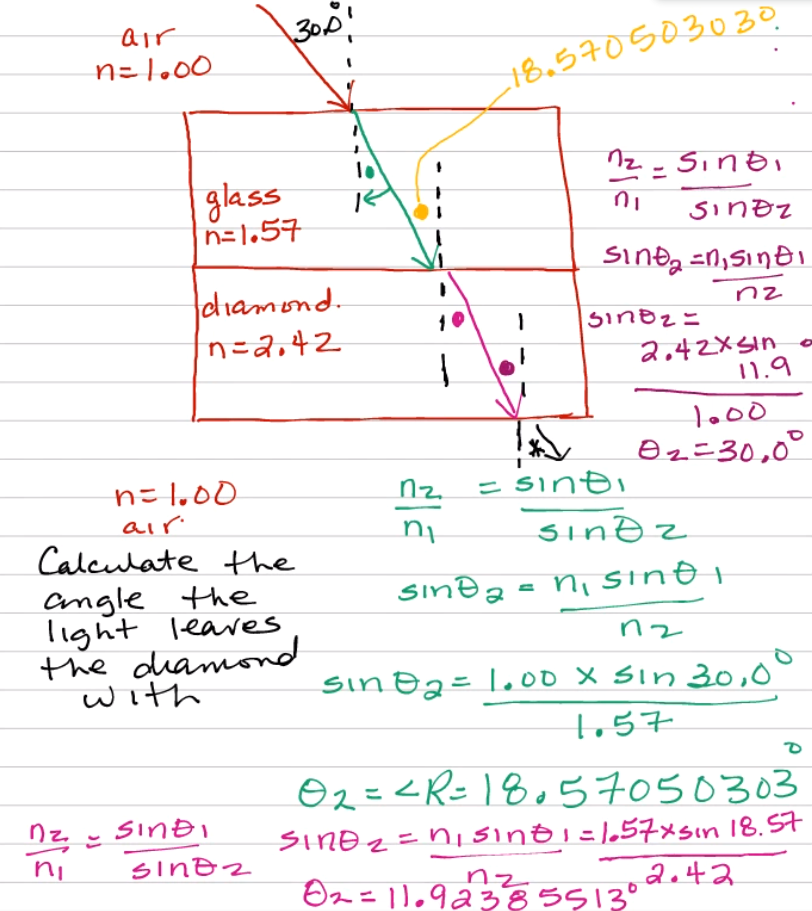
\includegraphics[width=\textwidth]{ex-sqr}
\end{figure}

\subsubsection{Equilateral Triangle}
\begin{figure}[H]
    \centering
    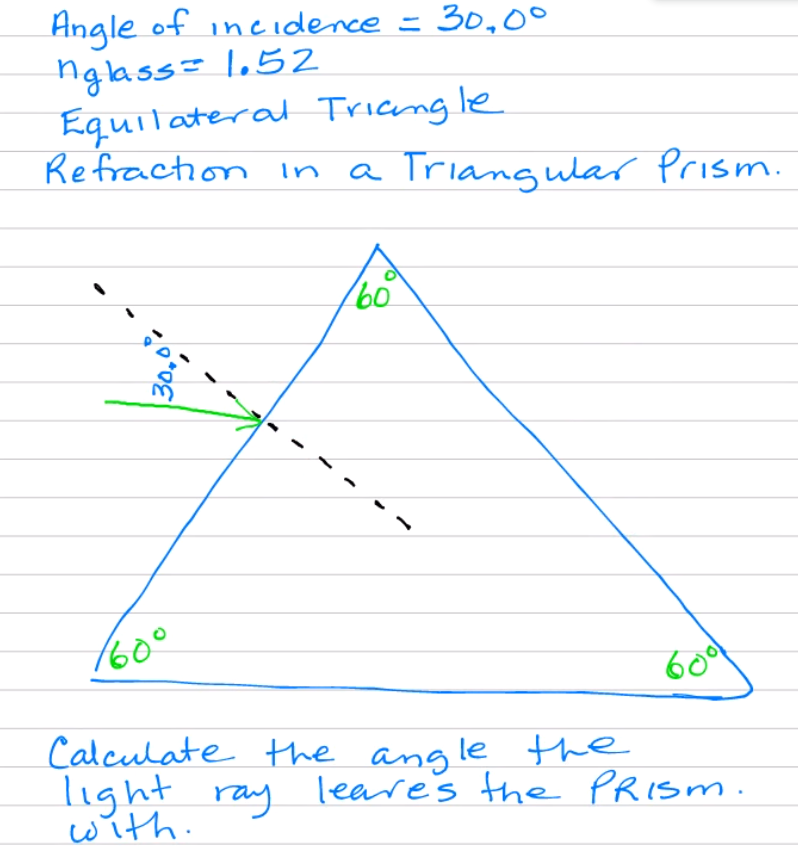
\includegraphics[width=0.45\textwidth]{ex-tri-1}
    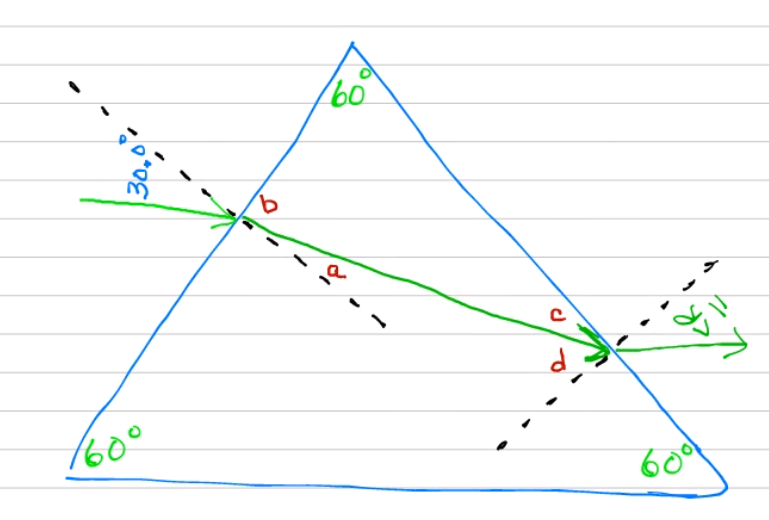
\includegraphics[width=0.45\textwidth]{ex-tri-2}
\end{figure}
\begin{figure}[H]
    \centering
    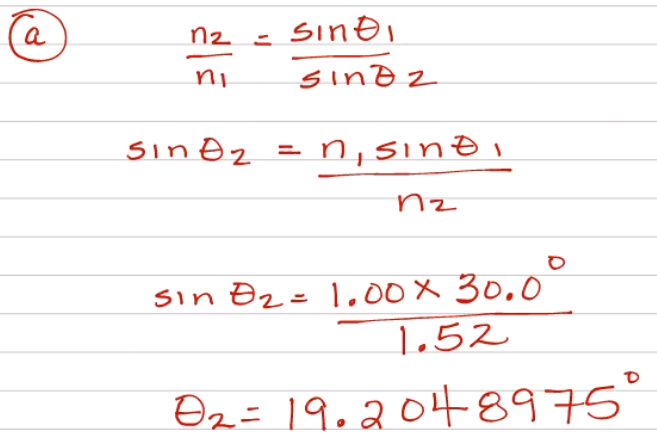
\includegraphics[width=0.45\textwidth]{ex-tri-3}
    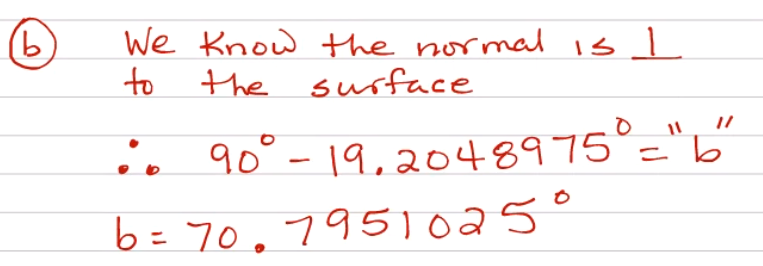
\includegraphics[width=0.45\textwidth]{ex-tri-4}
\end{figure}
\begin{figure}[H]
    \centering
    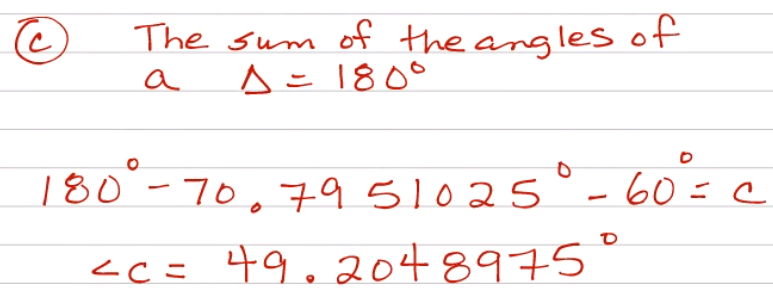
\includegraphics[width=0.45\textwidth]{ex-tri-5}
    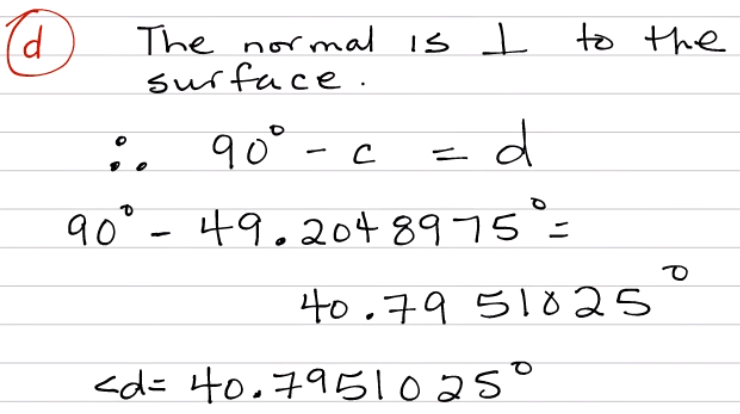
\includegraphics[width=0.45\textwidth]{ex-tri-6}
\end{figure}

$$\theta = \ang{83.3}$$

\pagebreak
\section{Dispersion}
\begin{figure}[H]
    \centering
    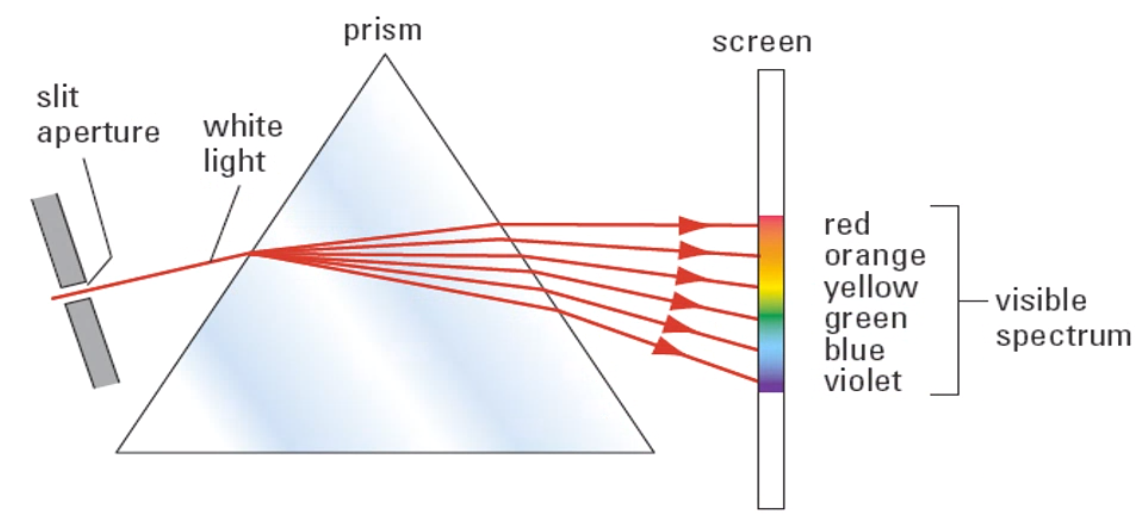
\includegraphics[width=0.8\textwidth]{dispersion}
\end{figure}

Separation of white light into its components.

The refraction of white light to form a spectrum of colours.

\textbf{Spectrum}: the bands of colours making up white light (red, orange, yellow, green, blue, violet)

In a rainbow, light from the sun enters a spherical raindrop and different colors are refracted at different angles.

\section{Ray Diagrams for Lenses}
\begin{itemize}
    \item{$f$: Focal length}
    \item{$m$: Magnification}
    \item{$d_o$: Object distance}
    \item{$d_i$: Image distance}
    \item{$h_o$: Object height}
    \item{$h_i$: Image height}
\end{itemize}

$$\frac{1}{f} = \frac{1}{d_o} + \frac{1}{d_i}$$
$$\frac{h_i}{h_o} = \frac{-d_i}{d_o}$$
$$m = \frac{d_i}{d_o}$$
$$m = \frac{h_i}{h_o}$$

$f$ is positive for convex lenses.
$f$ is negative for concave lenses.

\pagebreak
\section{Convex}
\begin{itemize}
    \item{Ray 1 starts from the top of the object and travels parallel to the principal axis until the light ray strikes the midline of the lens}
    \item{Ray 1 then bends and travels down through F}
    \item{Ray 2 starts at the top of the object and travels down through F until the rayt strikes the midline of the lens}
    \item{Ray 2 then refracts and travels parallel to the principal axis}
    \item{The light rays converge at a point}
\end{itemize}

\subsection{Object Beyond C}
aka. Converging Lens

\begin{figure}[H]
    \centering
    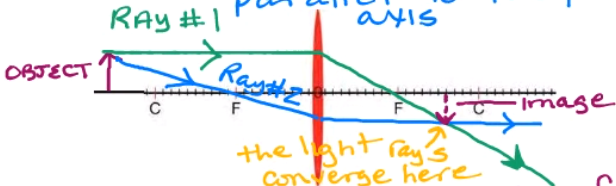
\includegraphics[width=0.8\textwidth]{convex}
\end{figure}

\hl{The resulting image can be described as...}
\begin{itemize}
    \item{\textbf{inverted} (upside down)}
    \item{\textbf{diminished} (smaller)}
    \item{located between F and C}
    \item{\textbf{real} (if the object and image are on opposite sides of the lens)}
\end{itemize}


\pagebreak
\subsubsection{Example}
A \SI{3.00}{\cm} tall object is placed \SI{30.0}{\cm} in front of a convex lens with a focal length of \SI{10.0}{\cm}. Calculate $d_i$, $h_i$ and $m$.
\begin{figure}[H]
    \centering
    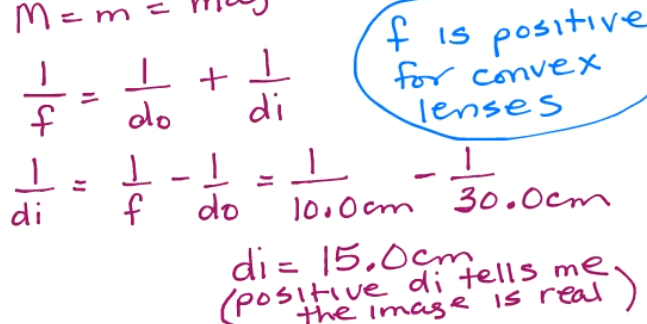
\includegraphics[width=0.45\textwidth]{ex-convex-1}
    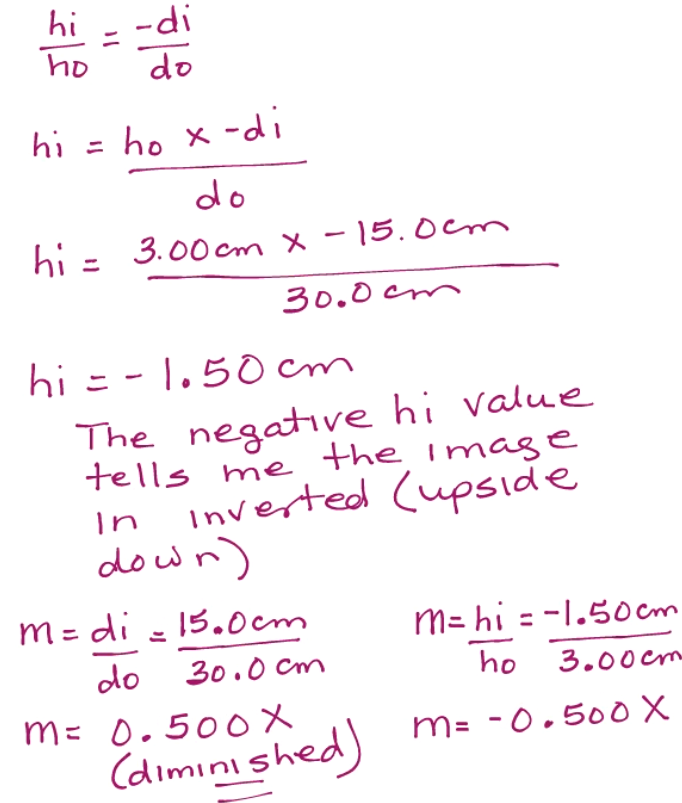
\includegraphics[width=0.45\textwidth]{ex-convex-2}
\end{figure}

\pagebreak
\subsection{Object At C}
\begin{figure}[H]
    \centering
    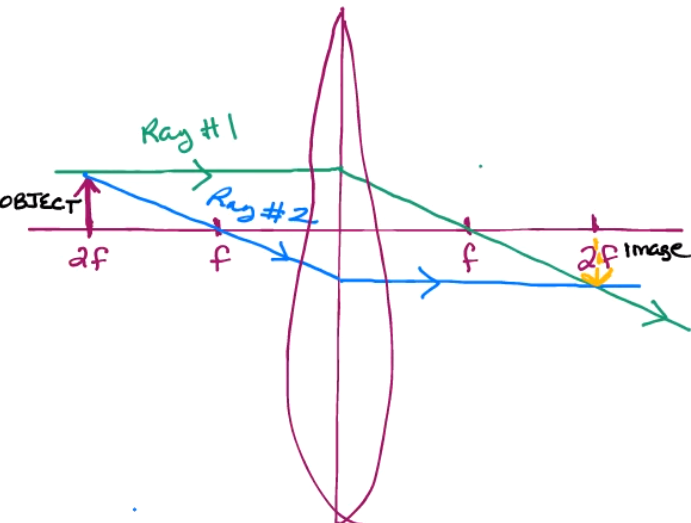
\includegraphics[width=0.75\textwidth]{convex-atc}
\end{figure}

\hl{The resulting image can be described as...}
\begin{itemize}
    \item{inverted}
    \item{same size}
    \item{located at C/2F}
    \item{real}
\end{itemize}

\pagebreak
\subsubsection{Example}
A \SI{2.00}{\cm} tall object is placed \SI{20.0}{\cm} in front of a convex lens with a focal length of \SI{10.0}{\cm}. Calculate $d_i$, $h_i$ and $m$.
\begin{itemize}
    \item{$h_o = \SI{2.00}{\cm}$}
    \item{$d_o = \SI{20.0}{\cm}$}
    \item{$f = \SI{10.0}{\cm}$}
\end{itemize}
$$\frac{1}{f} = \frac{1}{d_o} + \frac{1}{d_i}$$
$$\frac{1}{d_i} = \frac{1}{f} - \frac{1}{d_o}$$
$$\frac{1}{d_i} = \frac{1}{\SI{10.0}{\cm}} - \frac{1}{\SI{20.0}{\cm}}$$
$$d_i = \SI{20.0}{\cm}$$

$$\frac{h_i}{h_o} = \frac{-d_i}{d_o}$$
$$h_i = \frac{h_o \times -d_i}{d_o}$$
$$h_i = \frac{\SI{2.00}{\cm} \times \SI{-20.0}{\cm}}{\SI{20.0}{\cm}}$$

$$m = \frac{d_i}{d_o}$$
$$m = \frac{\SI{20.0}{\cm}}{\SI{20.0}{\cm}} = 1$$

\pagebreak
\subsection{Object between C and F}
\begin{figure}[H]
    \centering
    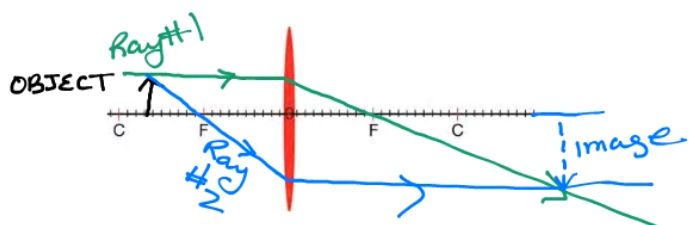
\includegraphics[width=0.8\textwidth]{convex-bfc}
\end{figure}

\hl{The resulting image can be described as...}
\begin{itemize}
    \item{inverted}
    \item{enlarged}
    \item{located beyond C/2F}
    \item{real}
\end{itemize}

\subsection{Object at F}
\begin{figure}[H]
    \centering
    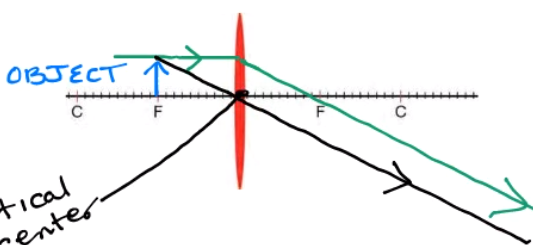
\includegraphics[width=0.7\textwidth]{convex-atf}
    \caption{Ray 2 cannot be used because the object is sitting on the focal point (F). We must use Ray 3.}
\end{figure}

Ray 3 (is an imaginary ray that) starts from the top of the object and travels down through the optical center of the lens. This ray does not refract.

The rays end up running parallel to each other, so there is \hl{no image}/\hl{image at infinity}.

\subsection{Convex, Object Inside F}
\begin{figure}[H]
    \centering
    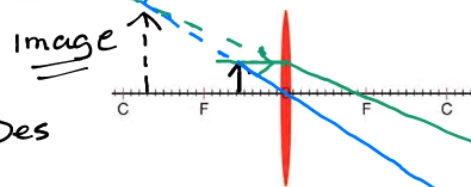
\includegraphics[width=0.7\textwidth]{convex-bf}
\end{figure}

\hl{The resulting image can be described as...}
\begin{itemize}
    \item{\textbf{erect} (right side up)}
    \item{enlarged}
    \item{located beyond C/2F}
    \item{\textbf{virtual} (object and image on same side)}
\end{itemize}

\subsubsection{Example}
A \SI{4.00}{\cm} tall object is \SI{20.0}{\cm} in front of a convex lens with a focal length of \SI{40.0}{\cm}. Calculate $d_i$, $h_i$ and $m$.
\begin{itemize}
    \item{$h_o = \SI{4.00}{\cm}$}
    \item{$d_o = \SI{20.0}{\cm}$}
    \item{$f = \SI{40.0}{\cm}$}
\end{itemize}
$$\frac{1}{f} = \frac{1}{d_o} = \frac{1}{d_i}$$
$$\frac{1}{d_i} = \frac{1}{f} - \frac{1}{d_o}$$
$$\frac{1}{d_i} = \frac{1}{\SI{40.0}{\cm}} - \frac{1}{\SI{20.0}{\cm}}$$
$$d_i = \SI{-40.0}{\cm}$$
Negative $d_i$ tells me the image is virtual.

$$\frac{h_i}{h_o} = \frac{-d_i}{d_o}$$
$$h_i = \frac{h_o \times -d_i}{d_o}$$
$$h_i = \frac{\SI{4.00}{\cm} \times -(\SI{-40.0}{\cm})}{\SI{20.0}{\cm}}$$
$$h_i = \SI{8.00}{\cm}$$
Positive $h_i$ means image is erect.

$$m = \frac{h_i}{h_o}$$
$$m = \frac{\SI{8.00}{\cm}}{\SI{4.00}{\cm}}$$
$$m = \num{2.00}$$
Image will be 2.00X bigger than object.

\pagebreak
\section{Concave}
\begin{itemize}
    \item{Diverging lens}
    \item{Ray 3 behaves as normal}
    \item{Ray 1 starts off straight and bends upward after the lens}
    \item{Use an imaginary line from point F to where ray 1 collides}
    \item{Ray 3 and the imaginary ray form the image}
\end{itemize}

\begin{figure}[H]
    \centering
    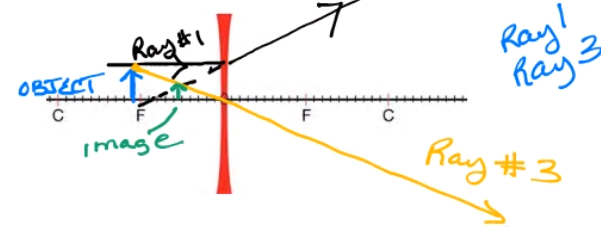
\includegraphics[width=0.75\textwidth]{concave-atf}
\end{figure}

\hl{Concave lenses ALWAYS result in images described as...}
\begin{itemize}
    \item{erect}
    \item{diminished}
    \item{virtual}
\end{itemize}

\subsection{Example}
A \SI{4.00}{\cm} tall object is \SI{15.0}{\cm} in front of a concave lens with a focal length of \SI{12.0}{\cm}. Calculate $d_i$, $h_i$, and $m$.
\begin{itemize}
    \item{$h_o = \SI{4.00}{\cm}$}
    \item{$d_o = \SI{15.0}{\cm}$}
    \item{$f = \SI{-12.0}{\cm}$}
\end{itemize}

$$\frac{1}{f} = \frac{1}{d_o} = \frac{1}{d_i}$$
$$\frac{1}{d_i} = \frac{1}{f} - \frac{1}{d_o}$$
$$\frac{1}{d_i} = \frac{1}{\SI{-12.0}{\cm}} - \frac{1}{\SI{15.0}{\cm}}$$
$d_i = \SI{-6.67}{\cm}$ (virtual)

$$\frac{h_i}{h_o} = \frac{-d_i}{d_o}$$
$$h_i = \frac{h_o \times -d_i}{d_o}$$
$$h_i = \frac{\SI{4.00}{\cm} \times -(\SI{-6.67}{\cm})}{\SI{15.0}{\cm}}$$
$h_i = \SI{1.78}{\cm}$ (erect)

$$m = \frac{h_i}{h_o}$$
$$m = \frac{\SI{1.78}{\cm}}{\SI{4.00}{\cm}}$$
$m = \num{0.444}$ (diminished)

\end{document}
